%%%%%%%%%%%%%%%%%%%%%%%%%%%%%%%%%%%%%%%%%
% Lachaise Assignment
% LaTeX Template
% Version 1.0 (26/6/2018)
%
% This template originates from:
% http://www.LaTeXTemplates.com
%
% Authors:
% Marion Lachaise & Fran�ois F�votte
% Vel (vel@LaTeXTemplates.com)
%
% License:
% CC BY-NC-SA 3.0 (http://creativecommons.org/licenses/by-nc-sa/3.0/)
% 
%%%%%%%%%%%%%%%%%%%%%%%%%%%%%%%%%%%%%%%%%

%----------------------------------------------------------------------------------------
%	PACKAGES AND OTHER DOCUMENT CONFIGURATIONS
%----------------------------------------------------------------------------------------

\documentclass{article}

%%%%%%%%%%%%%%%%%%%%%%%%%%%%%%%%%%%%%%%%%
% Lachaise Assignment
% Structure Specification File
% Version 1.0 (26/6/2018)
%
% This template originates from:
% http://www.LaTeXTemplates.com
%
% Authors:
% Marion Lachaise & Fran�ois F�votte
% Vel (vel@LaTeXTemplates.com)
%
% License:
% CC BY-NC-SA 3.0 (http://creativecommons.org/licenses/by-nc-sa/3.0/)
% 
%%%%%%%%%%%%%%%%%%%%%%%%%%%%%%%%%%%%%%%%%

%----------------------------------------------------------------------------------------
%	PACKAGES AND OTHER DOCUMENT CONFIGURATIONS
%----------------------------------------------------------------------------------------

\usepackage{amsmath,amsfonts,stmaryrd,amssymb} % Math packages

\usepackage{enumerate} % Custom item numbers for enumerations

\usepackage[ruled]{algorithm2e} % Algorithms

\usepackage[framemethod=tikz]{mdframed} % Allows defining custom boxed/framed environments

\usepackage{listings} % File listings, with syntax highlighting
\lstset{
	basicstyle=\ttfamily, % Typeset listings in monospace font
}

%----------------------------------------------------------------------------------------
%	DOCUMENT MARGINS
%----------------------------------------------------------------------------------------

\usepackage{geometry} % Required for adjusting page dimensions and margins

\geometry{
	paper=a4paper, % Paper size, change to letterpaper for US letter size
	top=2.5cm, % Top margin
	bottom=3cm, % Bottom margin
	left=2.5cm, % Left margin
	right=2.5cm, % Right margin
	headheight=14pt, % Header height
	footskip=1.5cm, % Space from the bottom margin to the baseline of the footer
	headsep=1.2cm, % Space from the top margin to the baseline of the header
	%showframe, % Uncomment to show how the type block is set on the page
}

%----------------------------------------------------------------------------------------
%	FONTS
%----------------------------------------------------------------------------------------

\usepackage[utf8]{inputenc} % Required for inputting international characters
\usepackage[T1]{fontenc} % Output font encoding for international characters

\usepackage{XCharter} % Use the XCharter fonts

%----------------------------------------------------------------------------------------
%	COMMAND LINE ENVIRONMENT
%----------------------------------------------------------------------------------------

% Usage:
% \begin{commandline}
%	\begin{verbatim}
%		$ ls
%		
%		Applications	Desktop	...
%	\end{verbatim}
% \end{commandline}

\mdfdefinestyle{commandline}{
	leftmargin=10pt,
	rightmargin=10pt,
	innerleftmargin=15pt,
	middlelinecolor=black!50!white,
	middlelinewidth=2pt,
	frametitlerule=false,
	backgroundcolor=black!5!white,
	frametitle={Command Line},
	frametitlefont={\normalfont\sffamily\color{white}\hspace{-1em}},
	frametitlebackgroundcolor=black!50!white,
	nobreak,
}

% Define a custom environment for command-line snapshots
\newenvironment{commandline}{
	\medskip
	\begin{mdframed}[style=commandline]
}{
	\end{mdframed}
	\medskip
}

%----------------------------------------------------------------------------------------
%	FILE CONTENTS ENVIRONMENT
%----------------------------------------------------------------------------------------

% Usage:
% \begin{file}[optional filename, defaults to "File"]
%	File contents, for example, with a listings environment
% \end{file}

\mdfdefinestyle{file}{
	innertopmargin=1.6\baselineskip,
	innerbottommargin=0.8\baselineskip,
	topline=false, bottomline=false,
	leftline=false, rightline=false,
	leftmargin=2cm,
	rightmargin=2cm,
	singleextra={%
		\draw[fill=black!10!white](P)++(0,-1.2em)rectangle(P-|O);
		\node[anchor=north west]
		at(P-|O){\ttfamily\mdfilename};
		%
		\def\l{3em}
		\draw(O-|P)++(-\l,0)--++(\l,\l)--(P)--(P-|O)--(O)--cycle;
		\draw(O-|P)++(-\l,0)--++(0,\l)--++(\l,0);
	},
	nobreak,
}

% Define a custom environment for file contents
\newenvironment{file}[1][File]{ % Set the default filename to "File"
	\medskip
	\newcommand{\mdfilename}{#1}
	\begin{mdframed}[style=file]
}{
	\end{mdframed}
	\medskip
}

%----------------------------------------------------------------------------------------
%	NUMBERED QUESTIONS ENVIRONMENT
%----------------------------------------------------------------------------------------

% Usage:
% \begin{question}[optional title]
%	Question contents
% \end{question}

\mdfdefinestyle{question}{
	innertopmargin=1.2\baselineskip,
	innerbottommargin=0.8\baselineskip,
	roundcorner=5pt,
	nobreak,
	singleextra={%
		\draw(P-|O)node[xshift=1em,anchor=west,fill=white,draw,rounded corners=5pt]{%
		Question \theQuestion\questionTitle};
	},
}

\newcounter{Question} % Stores the current question number that gets iterated with each new question

% Define a custom environment for numbered questions
\newenvironment{question}[1][\unskip]{
	\bigskip
	\stepcounter{Question}
	\newcommand{\questionTitle}{~#1}
	\begin{mdframed}[style=question]
}{
	\end{mdframed}
	\medskip
}

%----------------------------------------------------------------------------------------
%	WARNING TEXT ENVIRONMENT
%----------------------------------------------------------------------------------------

% Usage:
% \begin{warn}[optional title, defaults to "Warning:"]
%	Contents
% \end{warn}

\mdfdefinestyle{warning}{
	topline=false, bottomline=false,
	leftline=false, rightline=false,
	nobreak,
	singleextra={%
		\draw(P-|O)++(-0.5em,0)node(tmp1){};
		\draw(P-|O)++(0.5em,0)node(tmp2){};
		\fill[black,rotate around={45:(P-|O)}](tmp1)rectangle(tmp2);
		\node at(P-|O){\color{white}\scriptsize\bf !};
		\draw[very thick](P-|O)++(0,-1em)--(O);%--(O-|P);
	}
}

% Define a custom environment for warning text
\newenvironment{warn}[1][Warning:]{ % Set the default warning to "Warning:"
	\medskip
	\begin{mdframed}[style=warning]
		\noindent{\textbf{#1}}
}{
	\end{mdframed}
}

%----------------------------------------------------------------------------------------
%	INFORMATION ENVIRONMENT
%----------------------------------------------------------------------------------------

% Usage:
% \begin{info}[optional title, defaults to "Info:"]
% 	contents
% 	\end{info}

\mdfdefinestyle{info}{%
	topline=false, bottomline=false,
	leftline=false, rightline=false,
	nobreak,
	singleextra={%
		\fill[black](P-|O)circle[radius=0.4em];
		\node at(P-|O){\color{white}\scriptsize\bf i};
		\draw[very thick](P-|O)++(0,-0.8em)--(O);%--(O-|P);
	}
}

% Define a custom environment for information
\newenvironment{info}[1][Info:]{ % Set the default title to "Info:"
	\medskip
	\begin{mdframed}[style=info]
		\noindent{\textbf{#1}}
}{
	\end{mdframed}
}
 % Include the file specifying the document structure and custom commands
\usepackage{graphicx}
\usepackage{float}
%----------------------------------------------------------------------------------------
%	ASSIGNMENT INFORMATION
%----------------------------------------------------------------------------------------

\title{Single Molecule Simulation (SMS\_BP)} % Title of the assignment

\author{Baljyot Singh Parmar\\ \texttt{baljyot.parmar@mail.mcgill.ca}} % Author name and email address

\date{McGill University--- \today} % University, school and/or department name(s) and a date

%----------------------------------------------------------------------------------------

\begin{document}

\maketitle % Print the title

%----------------------------------------------------------------------------------------
%	INTRODUCTION
%----------------------------------------------------------------------------------------

\section*{Introduction} % Unnumbered section
The goal of the SMS\_BP package is 3 fold:
\begin{enumerate}
	\item Simulate motion of molecules with 3 properties:
	\begin{enumerate}
		\item Follow FBM (fractional brownian motion)
		\item Be bounded (3D by the cell boundary)
		\item Molecule motion can change in time based on some user input probability of change to/from states (allowable states are the Diffusivity ($\frac{\mu m ^{2}}{s^{\alpha}}$) and the Hurst exponent characterizing the correlations in the process' increments ($\alpha$).
	\end{enumerate}
	\item Model the motion of \textit{condensates} (and their size). This dictates a preferential location inside the cell where the probability of observing a molecule is higher than the rest of the cell. Multiple number of condensates can coexist and move independently. The probability of \textit{finding} a molecule is then set to a user defined value of the partition coefficient of the condensates.
	\item Combine these two underlying processes and create realistic Single Molecule Tracking Photoactivatible Localization Microscopy movies and images which can be used to train tracking methods or analysis methods for molecule trajectories and cluster detection. These need to incorporate the photo-physics of the probe used, along with the optics of the microscopy and camera detection. Namely, it needs to allow for:
	\begin{enumerate}
		\item motion blur
		\item defocus intensity decay
		\item defocus  PSF deformation
		\item blinking (ON/OFF) of the probe.
	\end{enumerate}
\end{enumerate}

\begin{info} % Information block
	This is not a technical document. I am not discussing how these features are implemented (i think i came up with really nice solutions and would love to talk about it) but to display the large functionality of this code base and how \textit{you} the user can interact with and use it for your own means. 
\end{info}

%----------------------------------------------------------------------------------------
%	PROBLEM 1
%----------------------------------------------------------------------------------------

\section{Simulation of Bounded FBM (n-dimensional)} % Numbered section

The first order of business is to confirm that SMS\_BP can simulate BM,FBM given some boundary. Here boundary conditions are implemented as reflecting. For the included plots im showing only 2D motion because it's easier to visualize but don't worry, the real simulation is 3D! In fact using the nice property of stationary increments of FBM you can use this to simulate n-dimensional motion (why you would want to do this I don't know, but you can)!

\begin{figure}[H]
	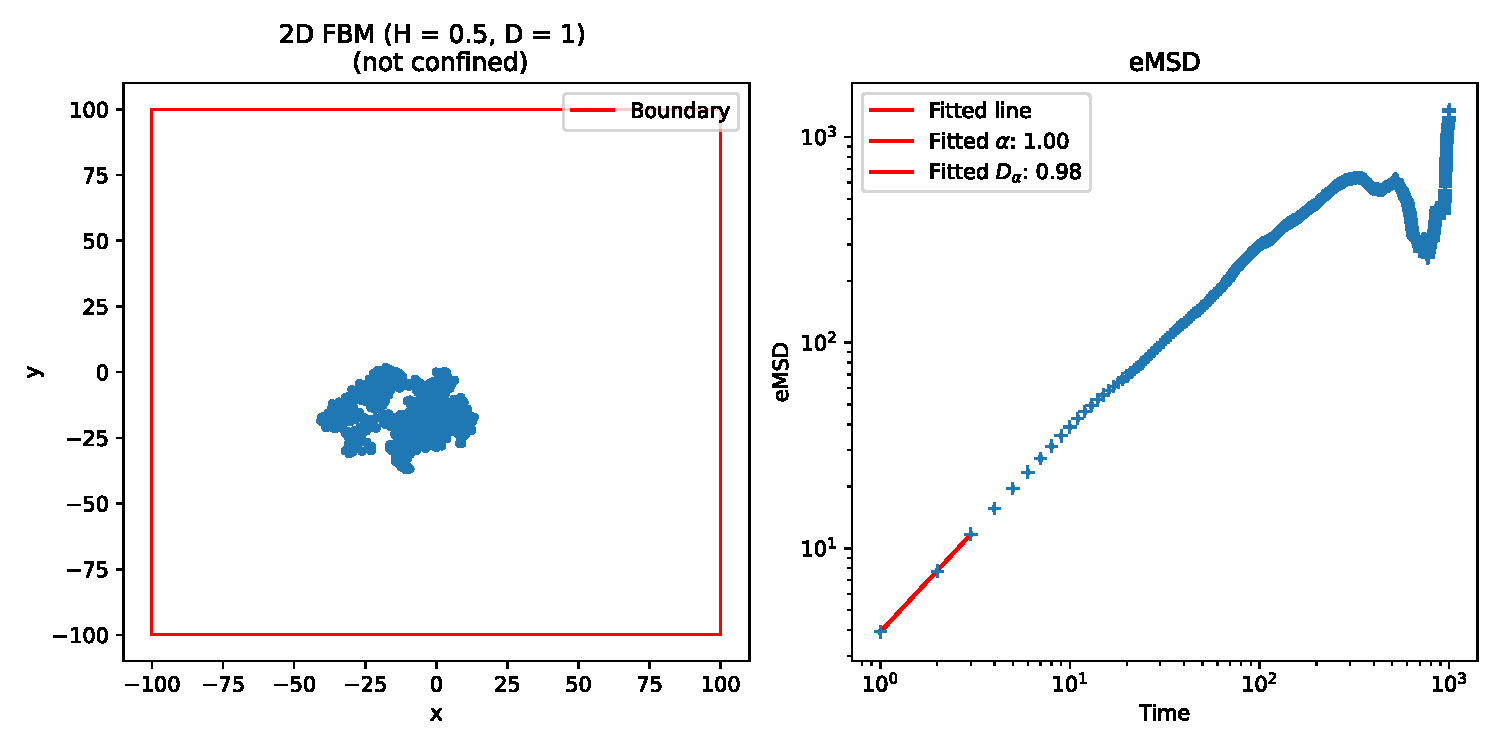
\includegraphics[width=1\textwidth]{Unconfined_Single_Motion_RANDOM.pdf}
	\caption{Example of an effectively unconfined random motion where the increments are so small and the duration is not large enough to encounter the boundary. We can simulate the correct D, $\alpha$! Don't worry the boundary is not set in stone and can be user defined. However it must be rectangular.}
\end{figure}

\begin{figure}[H]
	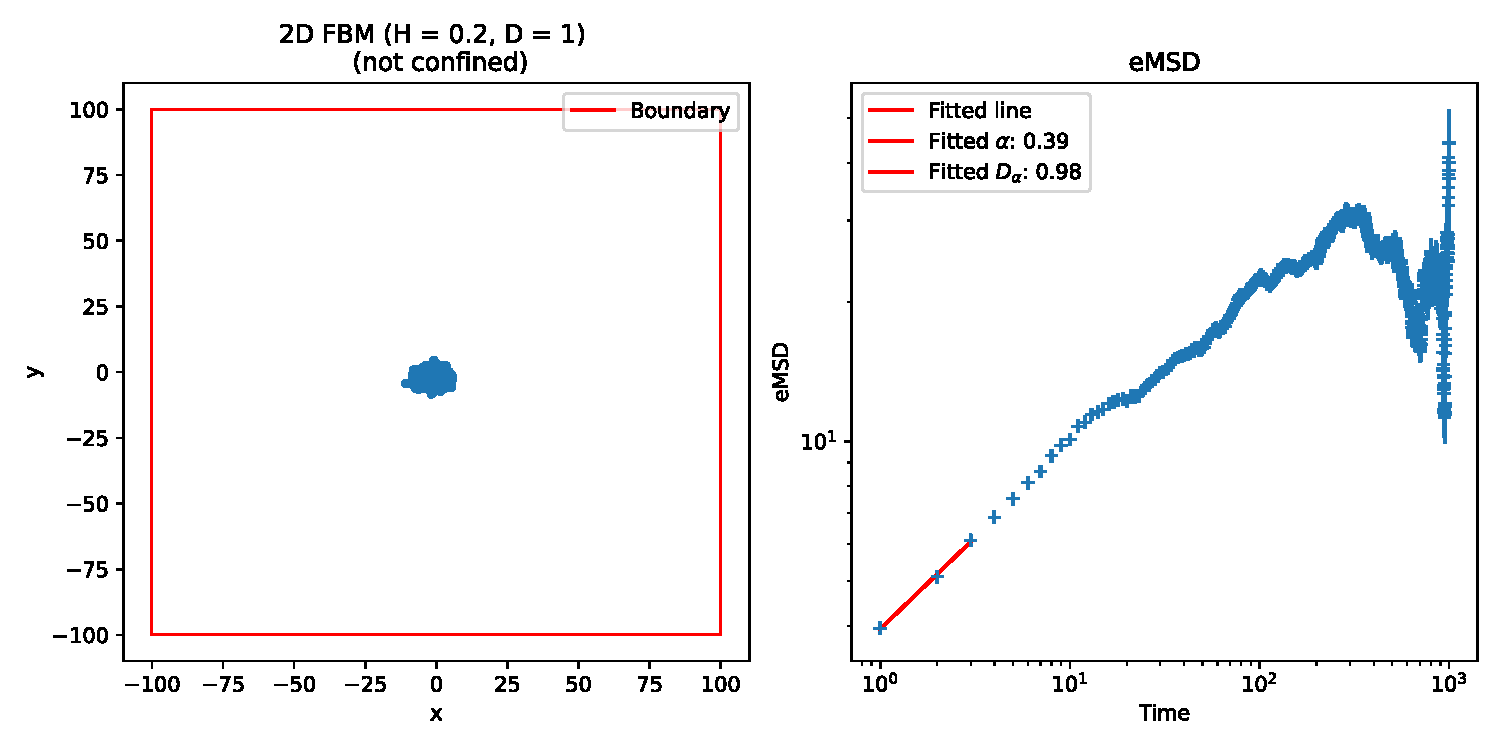
\includegraphics[width=1\textwidth]{Unconfined_Single_Motion_SUB.pdf}
	\caption{Example of an effectively unconfined subdiffusive motion where the increments are so small and the duration is not large enough to encounter the boundary. We can simulate the correct D, $\alpha$!}
\end{figure}

\begin{figure}[H]
	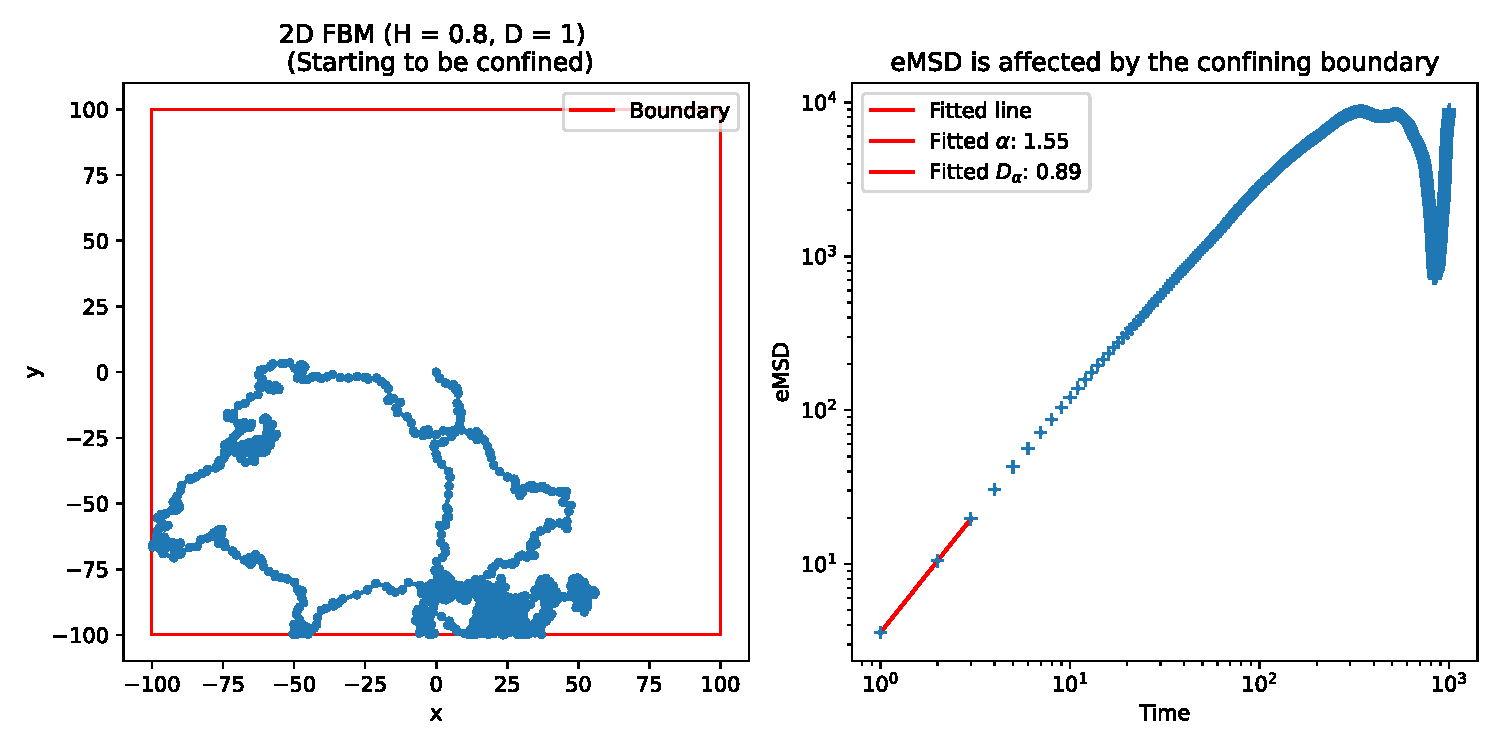
\includegraphics[width=1\textwidth]{Unconfined_Single_Motion_SUPER.pdf}
	\caption{Example of an confined superdiffusive motion where the increments are large enough to encounter the boundary. We can simulate the correct D, $\alpha$!}
\end{figure}
\begin{figure}[H]
	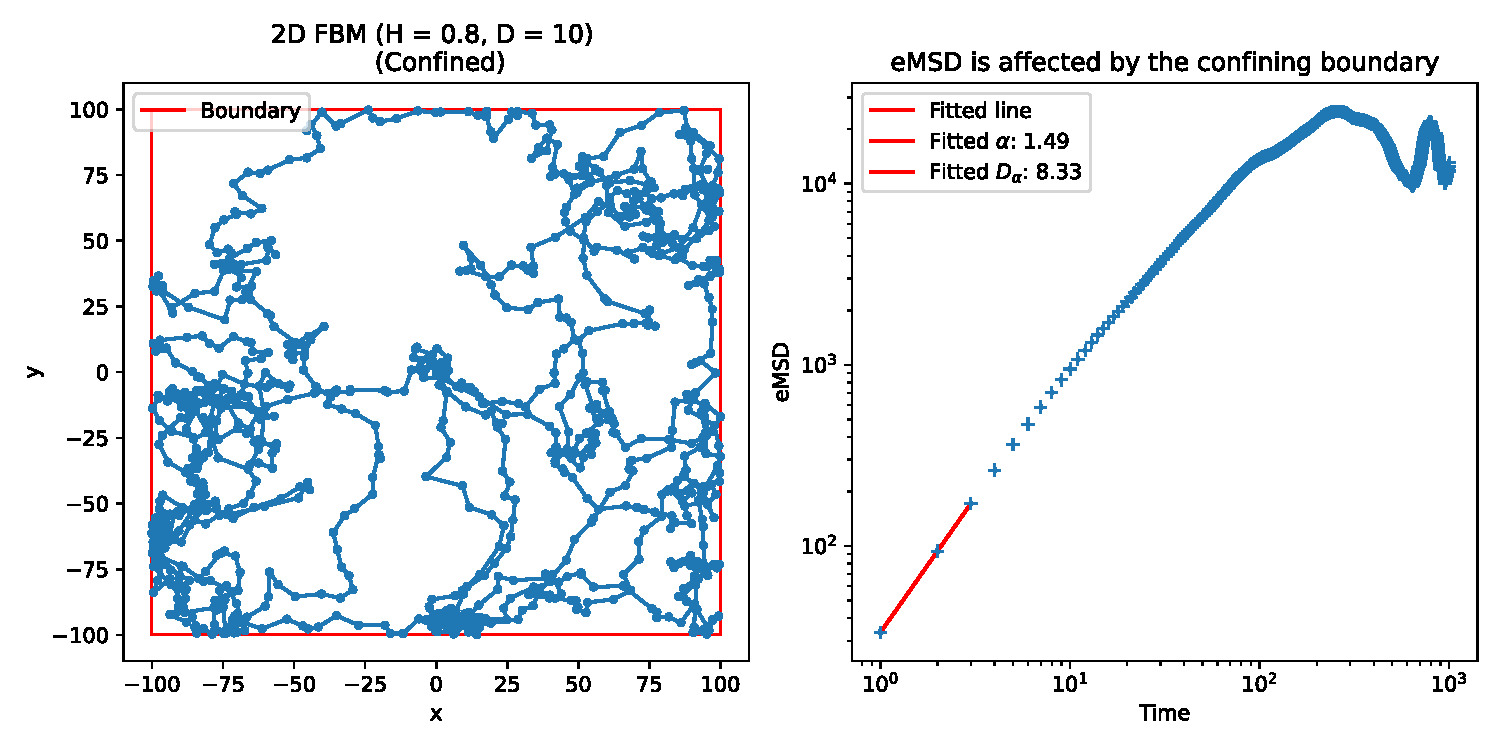
\includegraphics[width=1\textwidth]{Confined_Single_Motion_SUPER.pdf}
	\caption{Example of an confined superdiffusive motion where the increments are large enough to be totally confined by the boundary. We can simulate the correct D, $\alpha$ but the extracted fits suffer because of the interactions at the boundary interface!}
\end{figure}
\begin{figure}[H]
	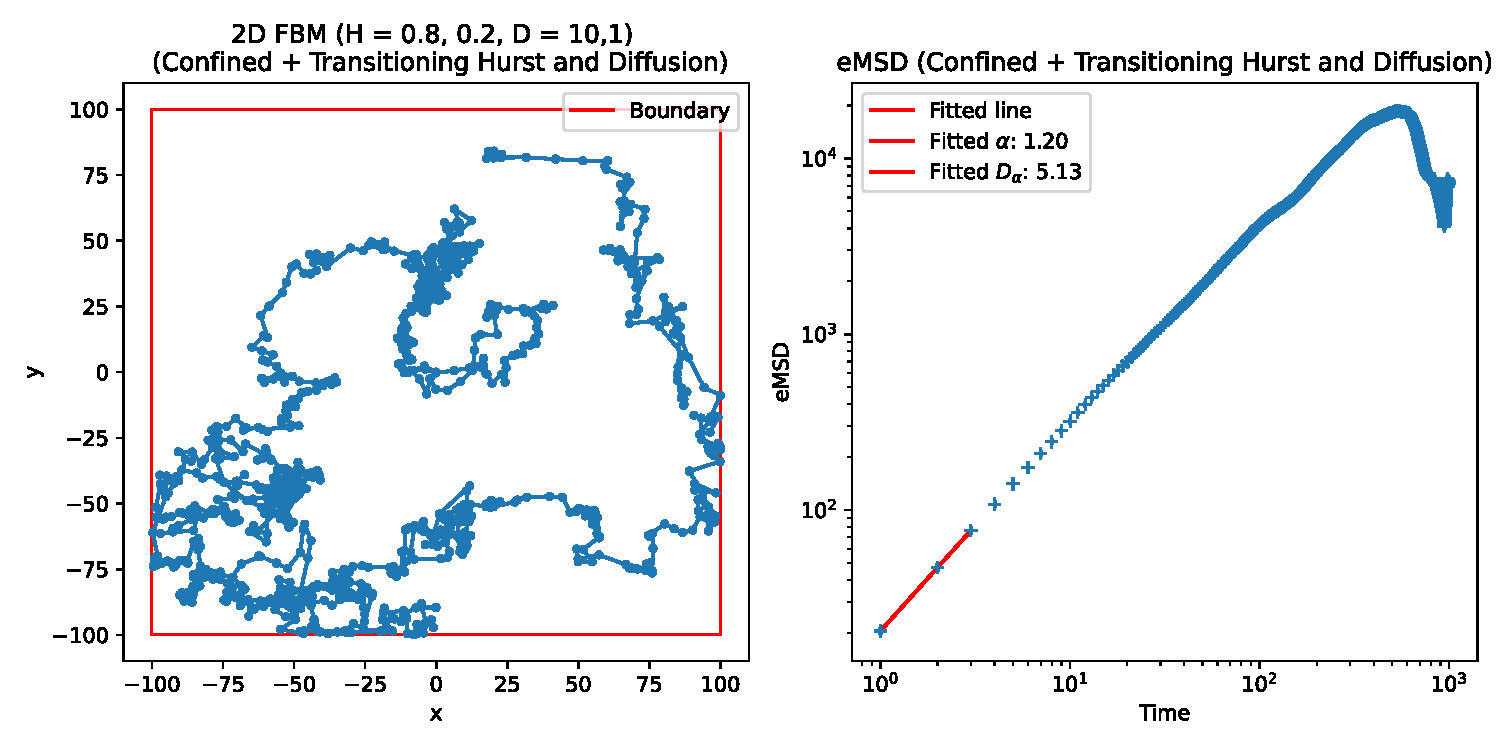
\includegraphics[width=1\textwidth]{Confined_Single_Motion_TRANSITIONING.pdf}
	\caption{Example of an confined transitioning motion. Here there are 4 states: 2 unique D, and 2 unique Hurst. The ensemble MSD is now a population average of for these and will greatly depend on the D,H values but also on the proportion of each state!}
\end{figure}
\begin{figure}[H]
	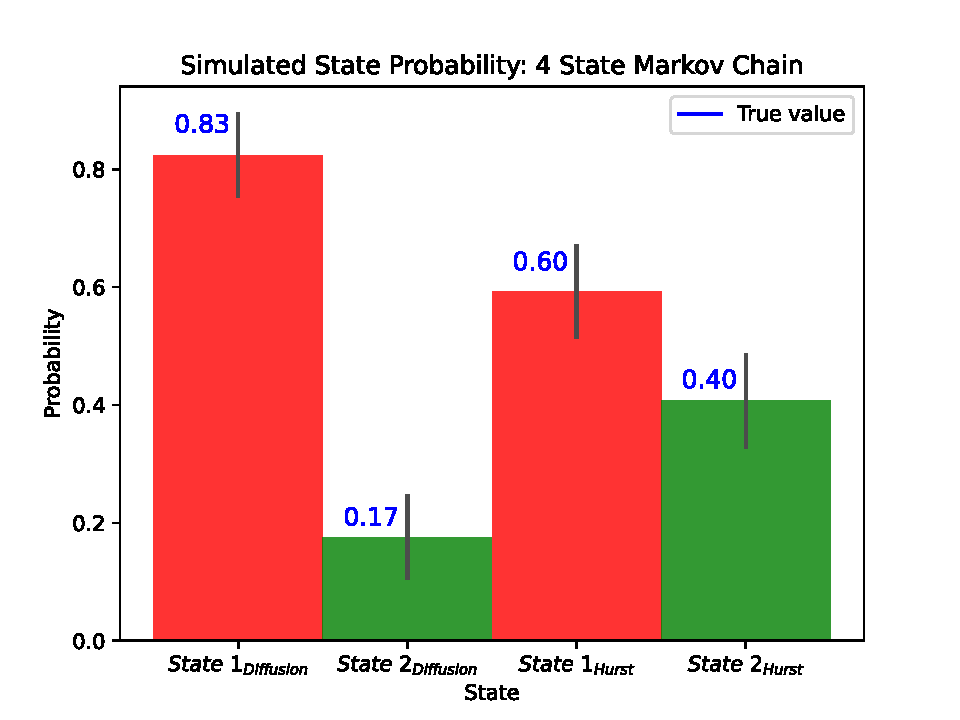
\includegraphics[width=0.5\textwidth]{state_probability.pdf}
	\caption{The example of Figure 5 showed the transitioning ability of the simulation. Here I show if the user (\textit{you}) gives the rates of transitioning from one state to another (and itself) SMS\_BP can accurately simulate the correct transitioning proportions. As a note, this is assuming the process is Markovian and as such is implemented under-the-hood as a MCMC (Markov chain monte carlo).}
\end{figure}

I want to emphasize that I only used 4 unique states here. In fact the user can ask for any combination of these (as many as you want) and the probabilities are all handled under-the-hood. You do not need to worry about typing anything other than the input parameters. I will discuss in future sections how you can define the parameters of the simulations and run it! By this point we have shown that the first goal is accomplished. Lets move on to the condensate!

\section{Condensate Definitions and Movement}
So far we have worked with individual trajectories and let them start at the origin. What if we want to simulate many trajectories (molecule motion) but starting at different places in the cells? One choice is to randomly sample the cellular space and start the observation of a molecule. But if the underlying space is heterogeneous in the density of molecules we are tracing we can define the cellular space as a probability space. Each spatial element defines the \textbf{expected} probability of finding a molecule in that region. This framework leads to the definition of a condensate!

A \textit{condensate} in the framework of SMS\_BP is defined as a circular/spherical region in the cell which has a higher probability per unit volume to find a molecule. That it, so simple! The nice consequence of using this simple definition is that we can also model the motion of the condensate by using the probability space. By letting the probability space be time dependent Figure 7 shows that we can treat the condensate as a moving trajectory itself and using the framework we developed previously to model its motion as BM or FBM! Isn't that cool? 
\begin{figure}[H]
	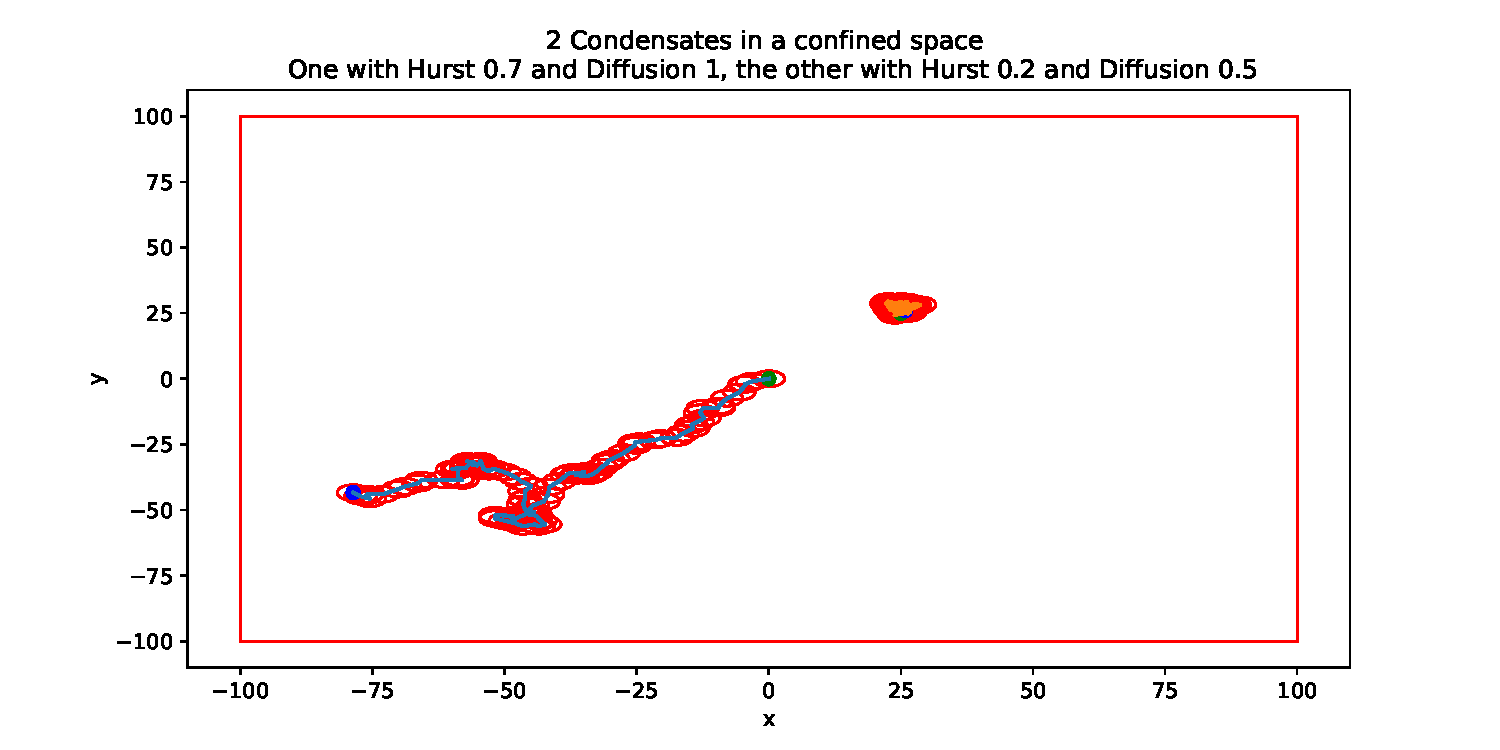
\includegraphics[width=1\textwidth]{Confined_Condensates.pdf}
	\caption{Here we can simulate any number of condensates (here I show 2). Implementation wise, their motion is independent of one another. But using the framework of the FBM from before we can model the condensates motion in anyway we like. Here one condensate is subdiffusive with a small diffusion coefficient and one which is super-diffusive with a larger diffusion coefficient. The blue lines represent the motion of the centre of each condensate. The red circles show the extent of the condensate boundary. In this case the size (radius) of the condensate does not change in time. But rest assured, SMS\_BP allows you to change this as you like! Since these objects are built on the same framework as the FBM, they share all the features of the molecule motion we outlined before.}
\end{figure}

Again you should think of the condensate as a probability space which is time and space dependent, $p(s,t)$. This condensate movement occurs in the background of the true molecule simulation and informs the location of the individual molecule positions as they \textit{turn on} to their fluorescent state. This is parameterized by a probability density  defined by the user which we will talk about later. For now bask in the glory that is SMS\_BP. 

\section{Conversion of Backend Trajectories to Observable PALM-like Images}

Okay all of the previous features are considered the backend of the simulation. They define what process are occurring. Our job now is to express these processes in a way which is similar to what an experimenter would observe from a typical SMT experiment. There are 3 things to consider: getting the photo-physics (intensities, PSF, etc ..) correct, modelling the effect of motion blurring, and the affect of the focal depth. 

The first is not that hard, assuming we have knowledge of the properties of the PSF and the intensities (photon counts) of individual molecule localizations (at a given exposure) we can define the mean photons emitted and captured at the detector in a time frame. The issue is the motion blurring. Since this is affected by fast motion and corresponding long exposures we actually sample the motion of the trajectories at a smaller time resolution than the exposure time! For example, if the exposure time is 100 ms the camera is on for 100 ms capturing photons emitted. Meanwhile the underlying molecule is still moving so rather than simulating the motion at 100 ms intervals we can simulate it at a smaller interval ($t < 100ms$) and integrate the photons over the exposure time, 100ms. For fast moving molecules which would resemble comet tails as the intensity (the photons) would \textit{leave} a trail of photons in its wake over the time the detector is on. 

SMS\_BP allows the user to define the smaller sample time, $t$. For example, in Figure 8 I show the effect of a sample time smaller than the exposure time. For visual aid I have cranked up the mean photons emitted/captured to make the comet tail readily apparent. You can change all these parameters, and we will do this in the final section. 

\begin{figure}[H]
	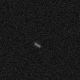
\includegraphics[width=0.5\textwidth, height=0.5\textwidth]{Cell_Movie_Test_001_Motion_Blur_high.png}
	\caption{Here the motion of a molecule is sampled every 1 ms. The exposure time is 20 ms and there is no interval time between measurements. All three of these parameters ca be user defined! Notice at this particualar frame the PSF of the molecule appears distorted? This is because of motion blur and defocus modelled by SMS\_BP. For visual aid I have artificially increased the mean photons emitted/captured for this molecule. The image is slightly ugly due to png compression, but you will get to make your own simulations and appreciate the details.}
\end{figure}
\begin{figure}[H]
	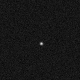
\includegraphics[width=0.5\textwidth, height=0.5\textwidth]{Cell_Movie_Test_001_noMotion_Blur_high.png}
	\caption{Here the motion of a molecule is sampled every 20 ms. The exposure time is 20 ms and there is no interval time between measurements. Notice there is no PSF deformation in this frame, since the molecule is modelled every 20 ms from the point of view of the simulation nothing occurs in the interval. This is because of there is no modelled motion blur and defocus by SMS\_BP. Compared to Figure 8 the only difference is that the over sampling (the $t$ I discuss in the text) is the \textbf{same} as the exposure time in this particular case. For visual aid I have artificially increased the mean photons emitted/captured for this molecule. }
\end{figure}

\section{Working With the Code}

First things first: use the installing instructions in the main README.md to get the conda environment created and the package installed on your system. This allows you to use the functionality of SMS\_BP from anywhere since the path is appended to the main python search path. 

There are 2 different ways to interact with the code. 
\begin{enumerate}
	\item The first is to use a configuration file which stores all the relevant parameters and passing it to a CLI-like file. The provided configuration file is sim\_config.json. The python file which takes this as an argument is called run\_cell\_simulation.
	\item The second is to use the actual code itself through import. We can do this since we have installed the code as a package.
\end{enumerate}

To keep it simple for now let's focus on the first method. Let's go to the config file in SMS\_BP/sim\_config.json and open it in your text editor of choice. You will see a nested dictionary with a bunch of parameters and associated values. We will go over each of these and what values are allowable. The document sim\_config.md is a text file describing each parameter and the units of each parameter in our main sim\_config.json. Use it as a reference if you want to change any of the parameters later on. 

First of all. Let's change one parameter in the sim\_config.json. Find the set of parameters called "Output\_Parameters". Inside you will find a parameter called "output\_path". Currently it contains a placeholder. Change this to a string which is the absolute path of the place you want SMS\_BP to store the final results. So to reiterate change the string \textbf{"<YOUR-PATH-HERE-CAN-BE-ABSOLUTE-OR-RELATIVE>"} to the path you want.

We can keep the rest of the parameters the same for now and let's just run the simulation. First way: run the run\_cell\_simulation.py by evoking \textbf{python run\_cell\_simulation.py sim\_config.json}. Else you can run it as: \textbf{python run\_cell\_simulation.py} and the logic will try to find the sim\_config.json file in the current directory. Once the simulation finishes you will find a new folder created at the path you specified and inside a few files and folders. For now ignore the folders. The .tiff file is the movie of the simulation. params\_dump.json is a copy of the sim\_config.json used to create this particular simulation, it is also provided as a pickle file. The final file Track\_dump.pkl is the true simulation of the underlying motion we did in section 1. This allows you to track the PSFs in the movie and compare back to the true positions of the molecules to see how well you did! 

Let's redo this but now with the variable oversample\_motion\_time equal to the exposure\_time. Set both to 20 (ms). Notice any difference in the two output movies? This is all I did to create figures 8-9.

To do further changes in the simulation I recommend reading the sim\_config.md file explaining the role of each parameter in the sim\_config.json file. If required I might make tutorials for other features I did not discuss here. 

%----------------------------------------------------------------------------------------

\end{document}
